\beginsong{Watt Ihr Volt}[wuw={Jakob Hoffmann, Kilian Hähn und Jonas Höchst}, jahr=2014, alb={BuLa 2014 - Watt ihr Volt}]

\newchords{verse}
\newchords{chorus}

% \beginverse\memorize[verse]
% \[D]Eulen habe Klasse, \[A]Eulen haben Stil,
% sie \[A7]können 1-A fliegen, und \[D]sagen nicht sehr viel.
% Bei \[B&]uns sind sie die Meister, der \[C]Kommunikation
% \[C]Immer nur Whats\[A]App, ganz echt: wer \[D]will das schon?
% \endverse
%
% \beginchorus\memorize[chorus]
% \[Gm]Abflug auf den Schachen, zehn \[A]Tage nächtelang...\[A] \[H] \[C#]
% Bei \[D]uns wird hart gerockt, bei \[A]uns wird sanft gerollt,
% bei \[G]uns gibt es ganz \[D]einfach \[A]Watt Ihr \[D]Volt!
% \endchorus

\beginverse
\endverse
\centering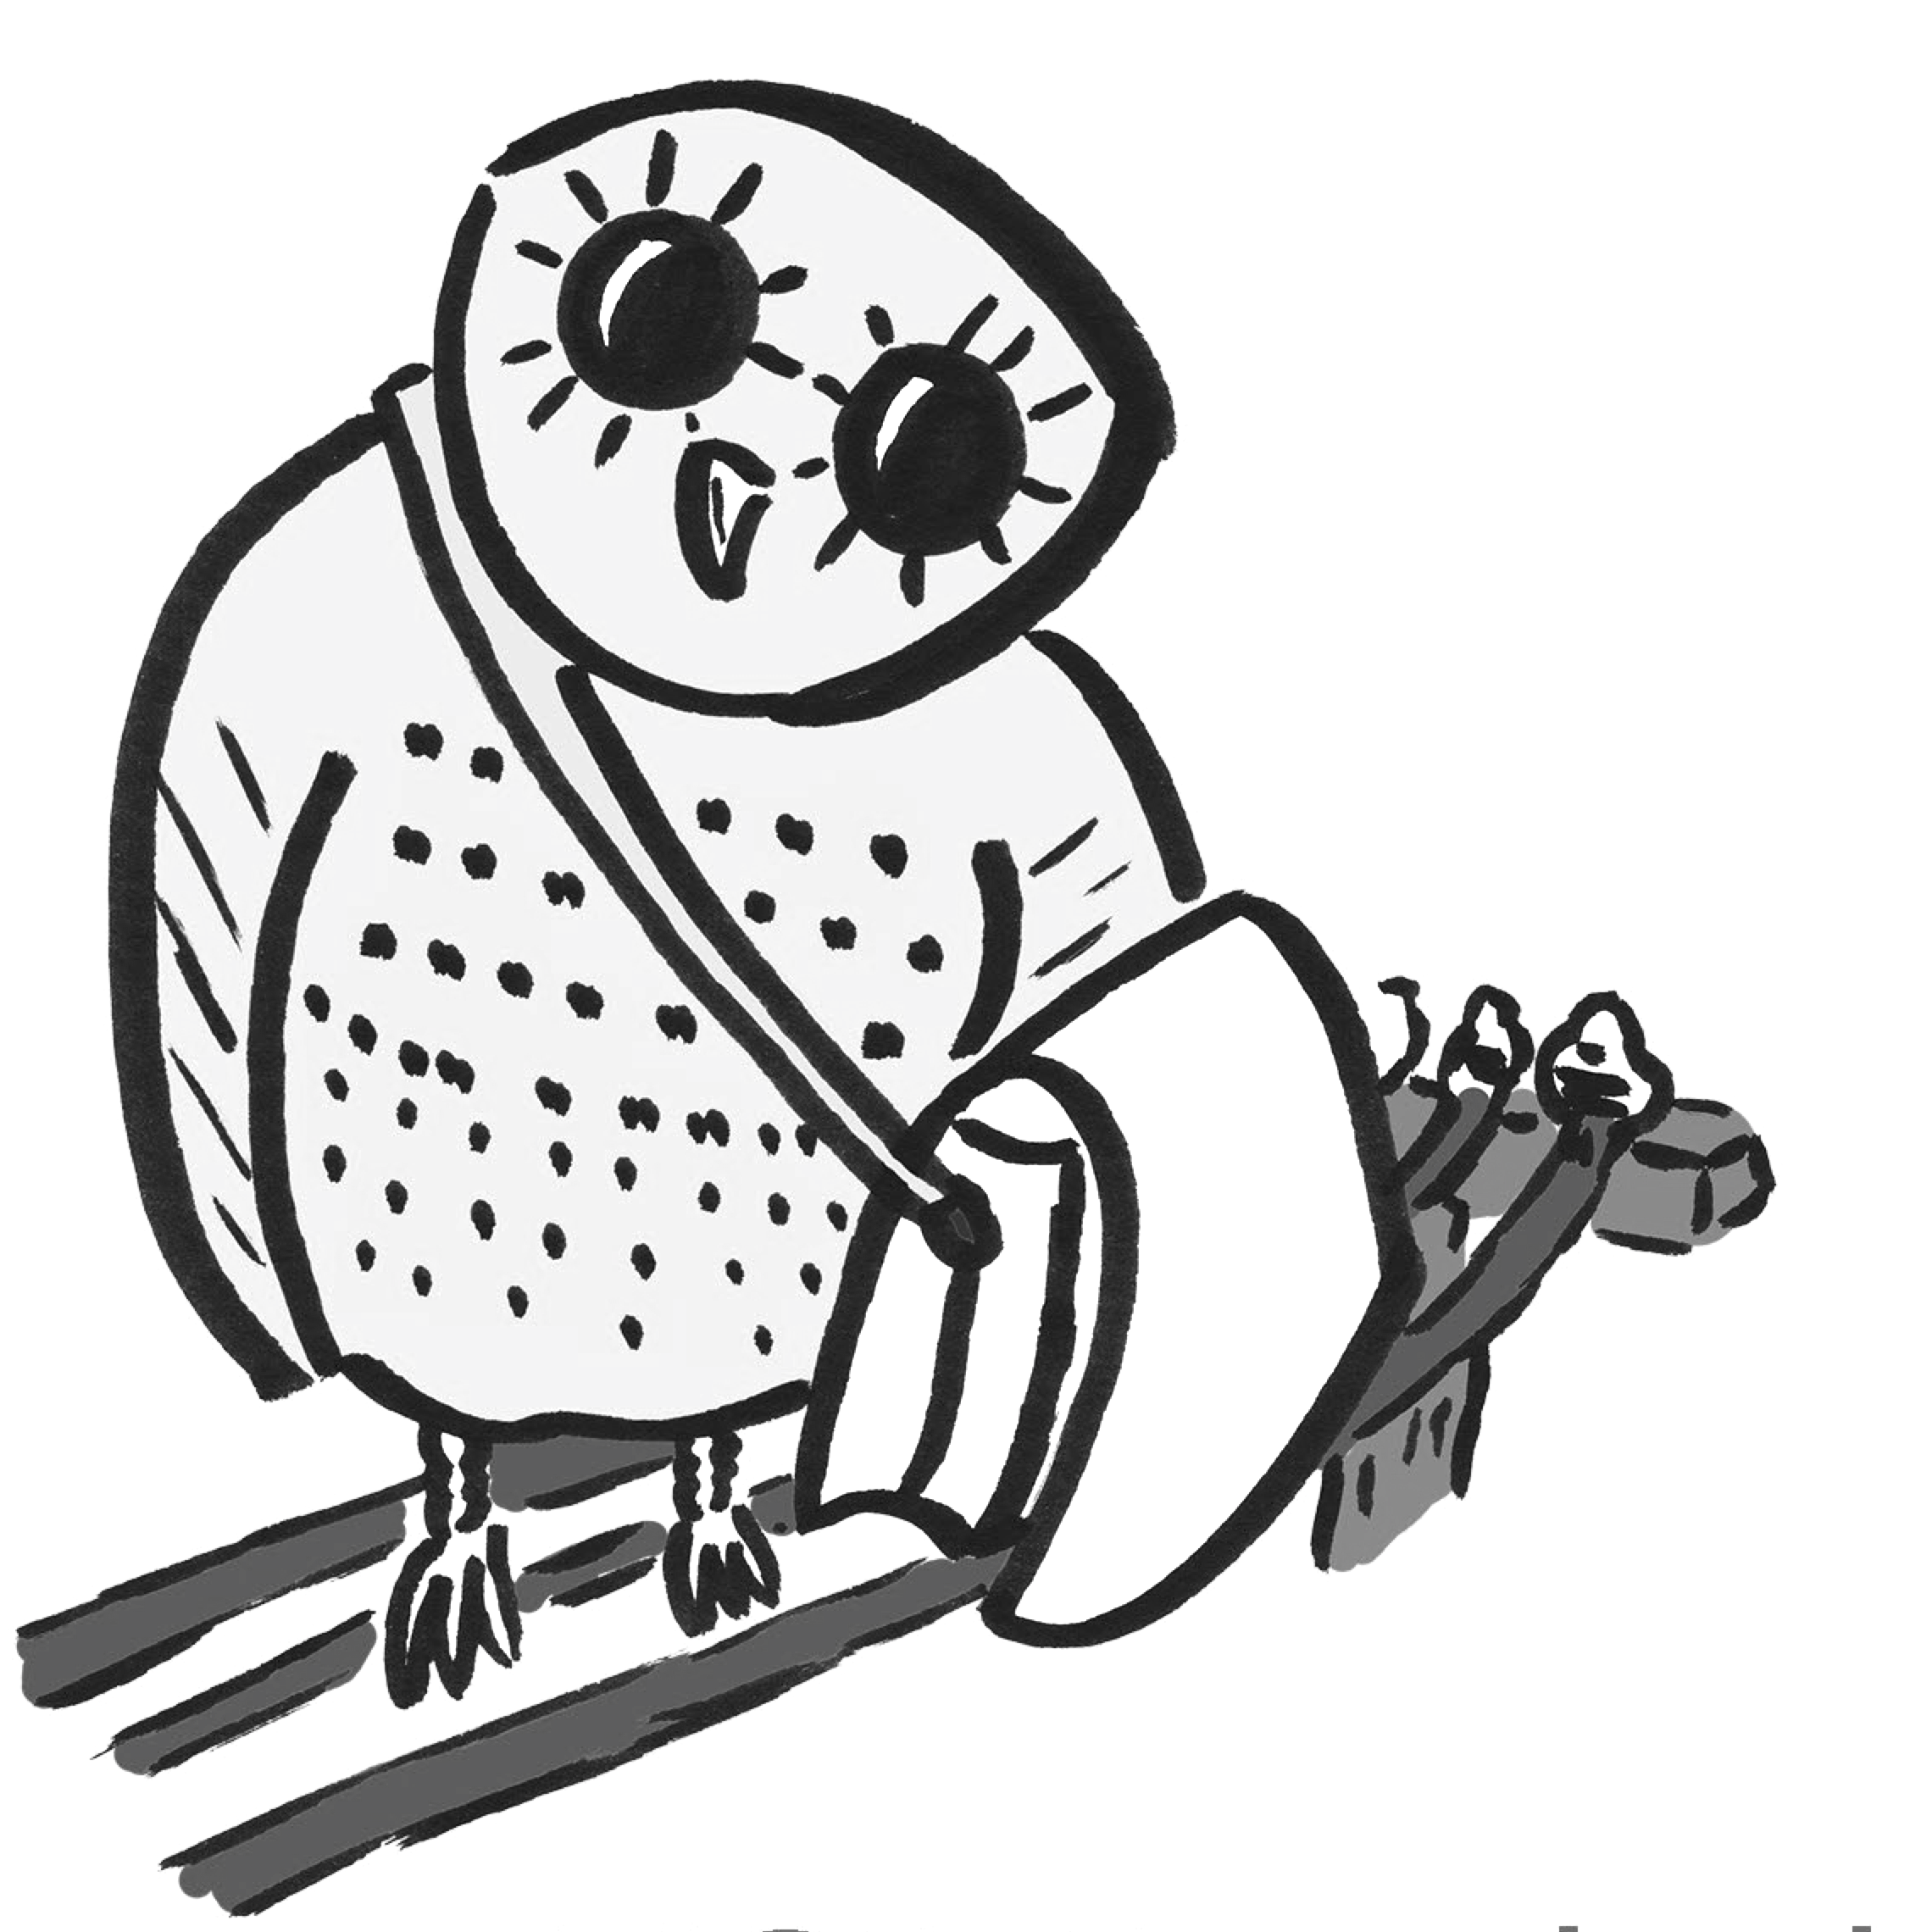
\includegraphics[width=1\textwidth]{Noten/WattIhrVolt.pdf}

\beginverse\memorize[verse]
Hier \[D]oben auf dem Hügel \[A]stehen wir im Wind.
\[A7]Er dreht unsere Räder, weil \[D]wir so clever sind.
\[B&]Selbst am neunten Abend hab'n \[C]wir noch Energie
Wir \[C]sind so eine \[A]Mischung aus \[D]Wahnsinn und Genie
\endverse

\beginchorus\memorize[chorus]
\[Gm]Abflug auf den Schachen, zehn \[A]Tage nächtelang... \[A] \[H] \[C#]
Bei \[D]uns wird nicht gejammert, bei \[A]uns wird nicht geschmollt,
wir \[G]feiern einfach \[D]alles \[A]Watt Ihr \[D]Volt!
\endchorus


\renewcommand{\everychorus}{\textnote{\bf Bridge im $\mathbf{\frac{3}{4}}$-tel Takt}}
\beginchorus\replay[verse]
Na^türlich gibt es Phasen, viel^leicht muss das so sein,
da ^sind wir schlaff und schweigsam und ^gerne mal allein. (\emph{Eins, zwo, drei, vier!})
Doch \[D]dann wird aus dem Koffer die \[A]Klampfe rausgeholt,
dann \[G]singt Ihr ganz ge\[D]nau das \[A]Watt Ihr \[D]Volt!
\endchorus
\renewcommand{\everychorus}{\textnote{\bf Refrain}}

\beginverse\replay[verse]
Was ^kümmert uns das Wetter? Was ^kratzt uns Dreck am Schuh?
^Was wir noch nicht können, er^finden wir dazu.
^Selbst den Dialekt hier ^ziehen wir uns rein:
''A ^bissle will doch ^jeder auch ein ^Schwabe sein!''
\endverse

\beginchorus\replay[chorus]
^Abflug auf den Schachen, zehn ^Tage nächtelang... ^ ^ ^
^Meistens scheint die Sonne und ^wenn der Himmel grollt,
zieh't ^euch was and'res ^an das ^Watt Ihr ^Volt!
\endchorus

\beginverse\replay[verse]
^Jeder kennt den Schock wenn ^man nach Hause kommt,
man ^schwebt mit Volldampf weiter, er^zählt voll Stolz davon,
wie's ^war auf diesem Lager, wie ^lustig wunderbar.
Doch ^raffen tut das ^keiner, der nicht ^oben war!
\endverse

\beginchorus\replay[chorus]
(Beim) ^Abflug auf den Schachen, zehn ^Tage nächtelang... ^ ^ ^
Was ^haben wir gerockt (haha), Was ^haben wir gerollt (haha)
Bei ^uns gab's einfach ^alles... \[D]Waaatt- \[A]iiihr- \[G]wooollt. \[D]
\endchorus

\endsong
\beginscripture{}
Geschrieben und Aufgenommen in $\mathit{7\frac{3}{4}}$ Anläufen auf dem Songwriting Wochenende im Frühsommer 2014. Zum Bundeslager Teillagerlied erkoren, zur heimlichen Hymne geworden!
\endscripture
